\begin{table*}[h!]
    \centering
    \caption{Ablation study for selecting which layers to project. The highlighted line with a blue rectangle is the setting used in DiZO. Extra memory indicates the extra memory needed due to pre-trained model storing. Attn\_Q: attention Query layer; Attn\_V: attention Value layer; Attn\_K: attention Key layer; Attn\_O: attention output projection; Dense: dense fully connected layer.}
    \vspace{5pt}
    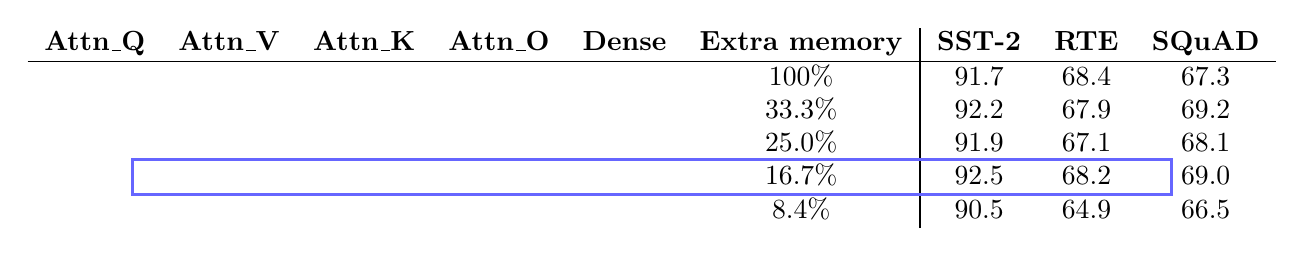
\begin{tikzpicture}
        \node (table) [inner sep=0pt] { % 嵌入表格
            \begin{tabular}{cccccc|ccc}
                \toprule
                \textbf{Attn\_Q} & \textbf{Attn\_V} & \textbf{Attn\_K} & \textbf{Attn\_O} & \textbf{Dense} & \textbf{Extra memory} & \textbf{SST-2} & \textbf{RTE} & \textbf{SQuAD} \\ \hline
                \cmark  & \cmark  & \cmark  & \cmark  & \cmark  & 100\%       & 91.7  & 68.4 & 67.3  \\
                \cmark  & \cmark  & \cmark  & \cmark  & \xmark  & 33.3\%      & 92.2  & 67.9 & 69.2  \\
                \cmark  & \cmark  & \cmark  & \xmark  & \xmark  & 25.0\%      & 91.9  & 67.1 & 68.1  \\
                \cmark  & \cmark  & \xmark  & \xmark  & \xmark  & 16.7\%      & 92.5  & 68.2 & 69.0  \\
                \cmark  & \xmark  & \xmark  & \xmark  & \xmark  & 8.4\%      & 90.5  & 64.9 & 66.5  \\
                \bottomrule
            \end{tabular}
        };

\draw[blue!60!white, very thick] (-6.6, -0.85) rectangle (6.6,-0.4);
    \end{tikzpicture}
    
    \label{ablation_layer}
\end{table*}